\documentclass[handout]{beamer}
\usepackage[utf8]{inputenc}
\usepackage[T1]{fontenc}
\usepackage[french]{babel}
\usepackage{color}
\usepackage{fancyhdr}
\usepackage{lmodern}
\usepackage{makeidx}
\usepackage{graphicx}
\usepackage{amsmath}
\usepackage{amssymb}
\usepackage{mathrsfs}
\usepackage[bottom]{footmisc}
\usepackage{float}
\usepackage{textcomp}
\usepackage{verbatim}
\usepackage{ulem}
\usepackage{xcolor}
\usepackage{subfig}

\usetheme{ki}
\usefonttheme{serif}

\title{Formation \LaTeX \vspace{0.2cm} Avancée}
\author{KI '020}
\institute{\color{white}Ecole des Ponts Paristech}
\date{\today}

\begin{document}

	\begin{frame}
		\titlepage
	\end{frame}

	\begin{frame}
		\frametitle{Sommaire}
		\setcounter{tocdepth}{1}
		\tableofcontents
	\end{frame}

\section{Rappels (?)}

	\begin{frame}
		\frametitle{Quelques Rappels ?}
		\begin{itemize}
			\item Bibliographie ?
		\end{itemize}
	\end{frame}

	\begin{frame}[fragile=singleslide]
		\frametitle{Bibliographie}

		\centering
		Fichier .bib :
		\begin{verbatim}
			@book{ArchitectureHydraulique,
title={Architecture Hydraulique,
Ou l'Art de Conduire, d'Élever Et de Ménager Les Eaux},
author={Bernard Forest de Bélidor},
year={1737},
publisher={Charles-Antoine Jombert}
}
		\end{verbatim}

	\end{frame}

	\begin{frame}[fragile=singleslide]
		\frametitle{Bibliographie}
		\centering
		Pour citer au milieu du texte :\\

		\begin{verbatim}
			Pour savoir quelle machine choisir, il est donc nécessaire
			de trouver un moyen de comparer deux machines (ou moteurs)
			entre elles : Navier veut une unité de mesure qui
			représenterait les "quantités de travail employées pour
			effectuer toute espèce de fabrication"
			\cite{ArchitectureHydraulique}.
		\end{verbatim}

	\end{frame}

	\begin{frame}[fragile=singleslide]
		\frametitle{Bibliographie}

		\centering
		Fichier .bib importé à la fin du document \LaTeX :
		\begin{verbatim}
			\bibliographystyle{plain}
			\bibliography{fichier.bib}
		\end{verbatim}

	\end{frame}

	\begin{frame}

		\centering

		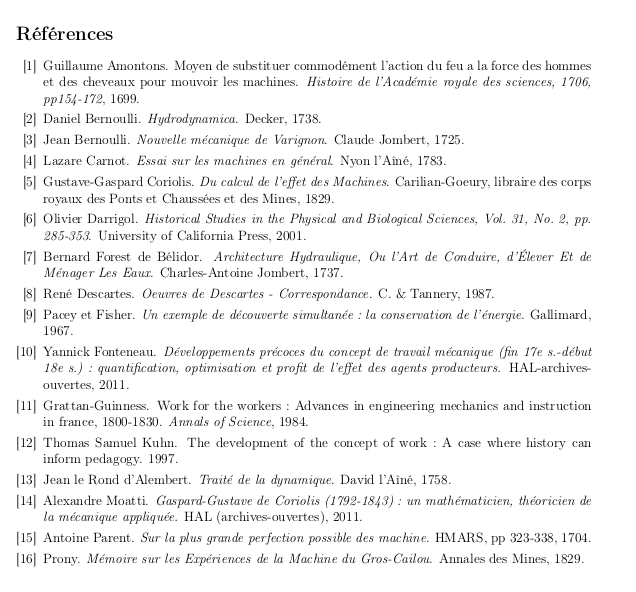
\includegraphics[scale=0.45]{Images/Rappels/biblio.png}

	\end{frame}

	\begin{frame}
		\frametitle{Quelques Rappels ?}
		\begin{itemize}
			\item Bibliographie ?
			\item Inclure des images (notamment des images côte à côte) ?
		\end{itemize}
	\end{frame}

	\begin{frame}[fragile=singleslide]
		\frametitle{Inclure des images}

		\centering
		\begin{verbatim}
			\begin{figure}[options de position]
				\caption{\label{etiquette} titre}
			\includegraphics[options sur l'image]{chemin}
		\end{figure}
		\end{verbatim}

		Liste d'options de position :
		\begin{itemize}
			\item \textit{h} à côté du texte précédent la source
			\item \textit{t} en haut d'une page
			\item \textit{b} en bas d'une page
			\item \textit{p} dans une page ne contenant que des \emph{flottants} (images, tableaux, etc.)
			\item Avec le package \textit{float}, on peut utiliser \textit{H}
		\end{itemize}

	\end{frame}

	\begin{frame}
		\frametitle{Inclure des images}

		\centering
		Mettre côte à côte : utiliser un environnement \textit{tabular}...
	\end{frame}

	\begin{frame}[fragile=singleslide]
		\frametitle{Inclure des images}

		\centering
		Mettre côte à côte : utiliser un environnement \textit{tabular}... ou de nouveaux packages !\\

		\begin{verbatim}
			\usepackage{subfig}
		\end{verbatim}

	\end{frame}

	\begin{frame}[fragile=singleslide]
		\frametitle{Inclue des images}

		\begin{verbatim}
			\begin{figure}[h]
  \begin{center}
	\subfloat[Coco \& Moi]{
	  \includegraphics[width=0.3\textwidth]{regiscoco1.jpg}
	  \label{sub:renonc}
						 }
	\subfloat[Moi \& Coco]{
	  \includegraphics[width=0.3\textwidth]{regiscoco2.jpg}
	  \label{sub:popul}
						 }
	\caption{C'était le WEI}
	\label{fig:renonculacees}
  \end{center}
\end{figure}
		\end{verbatim}

	\end{frame}

	\begin{frame}
		\frametitle{Inclure des images}

		\begin{figure}[h]
\begin{center}
\subfloat[Coco \& Moi]{
  \includegraphics[width=0.3\textwidth]{Images/Rappels/regiscoco1.jpg}
  \label{sub:renonc}
					 }
\subfloat[Moi \& Coco]{
  \includegraphics[width=0.3\textwidth]{Images/Rappels/regiscoco2.JPG}
  \label{sub:popul}
					 }
\caption{C'était le WEI}
\label{fig:renonculacees}
\end{center}
\end{figure}
	\end{frame}

	\begin{frame}
		\frametitle{Quelques Rappels ?}
		\begin{itemize}
			\item Bibliographie ?
			\item Inclure des images (notamment des images côte à côte) ?
			\item Manier des structures de tableaux ?
		\end{itemize}
	\end{frame}

\begin{frame}[fragile=singleslide]
	\frametitle{Tableaux}
	\centering
	Environnement \textit{tabular} :
	\begin{verbatim}
		\begin{tabular}{|l|c|r|}
			\hline
			colonne 1 & colonne 2 & colonne 3 \\
			\hline
			1 & 2 & 3\\
			\hline
		\end{tabular}
	\end{verbatim}

	\begin{tabular}{|l|c|r|}
		\hline
		colonne 1 & colonne 2 & colonne 3 \\
		\hline
		1 & 2 & 3\\
		\hline
	\end{tabular}

\end{frame}

\begin{frame}[fragile=singleslide]
	\frametitle{Tableaux}
	\centering
	Utilisation de \textit{multicolumn} :
	\begin{verbatim}
\begin{tabular}{|l|c|r|}
   \hline
   colonne 1 & \multicolumn{2}{c|}{colonnes 2 et 3} \\
   \hline
   1 & 2 & 3 \\
   \hline
   4 & 5 & 6 \\
   \hline
\end{tabular}
	\end{verbatim}

	\begin{tabular}{|l|c|r|}
	   \hline
	   colonne 1 & \multicolumn{2}{c|}{colonnes 2 et 3} \\
	   \hline
	   1 & 2 & 3 \\
	   \hline
	   4 & 5 & 6 \\
	   \hline
	\end{tabular}

\end{frame}

	\begin{frame}
		\frametitle{Quelques Rappels ?}
		\begin{itemize}
			\item Bibliographie ?
			\item Inclure des images (notamment des images côte à côte) ?
			\item Manier des structures de tableaux ?
			\item Environnement mathématique ?
		\end{itemize}
	\end{frame}

	\begin{frame}[fragile=singleslide]
		\frametitle{Mathématiques}

		\centering
		Environnement \textit{\$ \$}:
		\begin{verbatim}
			$\frac{a}{b} \leq \sqrt[n]{2}$
			$$ \iiint f(x,y,z)dxdydz $$
		\end{verbatim}

		$\frac{a}{b} \leq \sqrt[n]{2}$
		$$ \iiint_{\mathbb{R^3}} f(x,y,z)dxdydz $$

	\end{frame}

	\begin{frame}[fragile=singleslide]
		\frametitle{Mathématiques}
		\centering
		Environnement \textit{align, equation} :
		\begin{verbatim}
			\begin{equation}
				\cos(z)^2+\section(z)^2 \neq 0
			\end{equation}
		\end{verbatim}

		\begin{equation}
			\cos(z)^2+\sin(z)^2 \neq 0
		\end{equation}


	\end{frame}

	\begin{frame}[fragile=singleslide]
		\frametitle{Mathématiques}
		\centering
		\begin{verbatim}
			\begin{align}
				\mathbb{E}(Z)
				&= \frac{1}{n}\sum_{i=1}^n \mathbb{E}(1)
				&= \exp(0)
			\end{align}
		\end{verbatim}

		\begin{align}
			\mathbb{E}(Z)
			&= \frac{1}{n}\sum_{i=1}^n \mathbb{E}(1)\\
			&= \exp(0)
		\end{align}

	\end{frame}

	\begin{frame}
		\frametitle{Quelques Rappels ?}
		\begin{itemize}
			\item Bibliographie ?
			\item Inclure des images (notamment des images côte à côte) ?
			\item Manier des structures de tableaux ?
			\item Environnement mathématique ?
			\item Les bonnes pratiques pour travailler en groupe ?
		\end{itemize}
	\end{frame}

	\begin{frame}
		\frametitle{Quelques Rappels ?}
		\begin{itemize}
			\item Bibliographie ?
			\item Inclure des images (notamment des images côte à côte) ?
			\item Manier des structures de tableaux ?
			\item Environnement mathématique ?
			\item Les bonnes pratiques pour travailler en groupe ?
			\item Se servir d'un moteur de recherche ?
		\end{itemize}
	\end{frame}

\section{Faire de \emph{magnifiques} slides}

\section{Utiliser des templates}

\section{Mettre des gifs animés dans les slides ?}



\end{document}
